\chapter{Introduction}

Each year, the robotic community gathers at conferences such as IROS
(International Conference on Intelligent Robots and Systems), where they
exhibit their discoveries and achievements in the field. For the year 2019, the
Drone Racing League will be hosting a series of races which autonomous drones
will compete and attempt to outperform a professional drone pilot.\\
\begin{figure}[h]
	\centering
	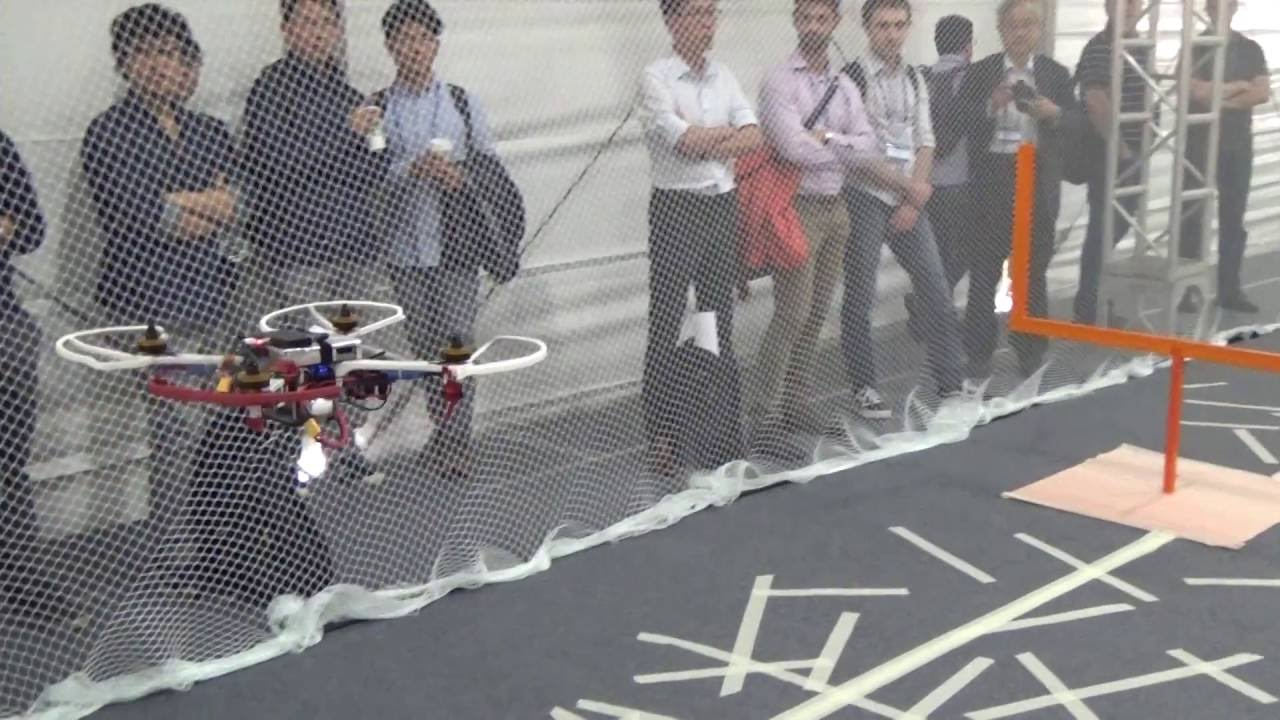
\includegraphics[width=0.5\textwidth]{figure/iros_2016.jpg}
	\caption{Drone racing arena at IROS 2016.}
	\label{fig:iros}
\end{figure}
The company Lockheed Martin is sponsoring the event and offering a prize of 2
million USD for the winning team. Teams of university students and other drone
enthusiasts shall present innovative approaches on vision-based systems for
unmanned aerial vehicles: hence, they showcase their progress through racing.\\

\todo{Talk about the predictions for AI in drone racing and drones in general
for the future}


Most robotic system's operation can be modeled by the commonly known
\emph{Sense, Plan, Act} paradigm:
\todo{Add custom act, sense, plan paradigm picture}
\begin{figure}[h]
	\centering
	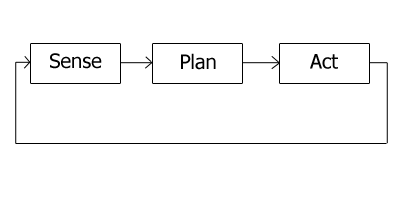
\includegraphics[width=0.4\textwidth]{figure/robotic_paradigm.png}
	\caption{The Sense, Plan, Act robotic paradigm.}
	\label{fig:robotic_paradigm}
\end{figure}

\begin{itemize}
	\item{\textbf{Sense}}: gather information using sensors (camera, IMU, sonar...).
	\item{\textbf{Plan}}:create a world model using all the information, and plan
		the nextmove.
	\item{\textbf{Act}}: carry out the actions that the plan calls for.
\end{itemize}
~\\
This thesis will be focused mainly on the sensing of the drone control, and
more precisely using computer vision algorithms along with machine learning
concepts. However, an important part of the trajectory planning directly
follows the sensing phase, therefore those two first phases of the control loop
can be included in the scope of the project.

To this day, most drones in the robotic research field are running \emph{Robot
Operating System} (ROS) \todo{Add citation}, which is a set of "libraries and
tools to help software developers create robot applications". The implementation
of the computer vision algorithms will be constrained within ROS, and cooperate
with the different control components provided by the project team.\\

\todo{Talk about why CNNs are used more and more in drone racing, and basically
why it is the chosen approach, which leads to tackling the dataset generation
problem.}

As Deep Learning has known an exponential growth during the past decade,
computer vision applications tend to exploit the power of convolutional neural
networks more and more. Thanks to their impressive accuracy in specific problem
solving, CNNs are becoming the main choice for tasks such as: object detection,
object segmentation, object recognition, \emph{etc}\ldots

In drone racing, the latest works, which are often the best performing, tend to
employ CNNs for the sensing part, or even as an all-in-one solution (refer to
\todo{refer to litterature review}).\\


The solution will be implemented iteratively, by gradually increasing the
complexity of the vision algorithms, such that progress can be made even if the
end goal is too difficult to achieve.\\

The project should attempt to fulfill the following goals:

\begin{itemize}
	\item{Recognize gates in the input image}
	\item{Detect and localize the closest gate's center}
	\item{Evaluate the closest gate's orientation and distance}
	\item{Plan a trajectory for the drone to fly across the gate center}
	\item{Refine the trajectory in real time, for an optimal flight time}
	\item{Make the drone follow that trajectory while adjusting in real time}
\end{itemize}
~\\
However, the following functionalities are out of the scope and will be
discarded:

\begin{itemize}
	\item{Detect any other obstacles in the input image}
	\item{Avoid obstacles that are on the drone's trajectory}
	\item{Map and localize the detected gates in world frame}
	\item{Plan a trajectory of a sequence of gates}
	\item{Apply online learning for adaptive racing}
\end{itemize}


~\\
The focus of this research will be on developing a robust and generalized
vision algorithm for detecting obstacles in a configurable manner and regardless
of their shape and color, such that the race gates can be specified prior to the
training of the algorithm, and thus tailored to the challenge itself. The end
goal is to greatly facilitate the learning of the vision-based detection model,
by automating the tedious and long process of collecting and annotating a large
dataset required to train the object detection algorithm using Deep Learning.

Indeed, this task is often the most time-consuming part of training
convolutional neural networks, mostly because each image must be annotated to be
used in supervised learning. By removing this weight off researchers' shoulders,
much more time is left to focus and experiment on the \emph{planning} and
\emph{acting} problems of the robotic paradigm \todo{reference to the diagram
above}.

In this work, the efficiency and robustness of tailored dataset generation for
Deep Learning-based computer vision algorithms, for the specific case of
autonomous drone racing, is analysed and discussed.
A simple approach to solving the \emph{planning} challenge is also undertaken,
which supports the praises of the proposed solution.
